% options:
% thesis=B bachelor's thesis
% thesis=M master's thesis
% czech thesis in Czech language
% slovak thesis in Slovak language
% english thesis in English language
% hidelinks remove colour boxes around hyperlinks

\documentclass[thesis=M,czech]{FITthesis}[2012/06/26]

\usepackage[utf8]{inputenc} % LaTeX source encoded as UTF-8

\usepackage{float}

\usepackage{graphicx} %graphics files inclusion
% \usepackage{amsmath} %advanced maths
% \usepackage{amssymb} %additional math symbols

\usepackage{dirtree} %directory tree visualisation

% % list of acronyms
% \usepackage[acronym,nonumberlist,toc,numberedsection=autolabel]{glossaries}
% \iflanguage{czech}{\renewcommand*{\acronymname}{Seznam pou{\v z}it{\' y}ch zkratek}}{}
% \makeglossaries

\newcommand{\tg}{\mathop{\mathrm{tg}}} %cesky tangens
\newcommand{\cotg}{\mathop{\mathrm{cotg}}} %cesky cotangens

% % % % % % % % % % % % % % % % % % % % % % % % % % % % % % 
% ODTUD DAL VSE ZMENTE
% % % % % % % % % % % % % % % % % % % % % % % % % % % % % % 

\department{Katedra softwarového inženýrství}
\title{Vývoj FIORI aplikace nad SAP PM modulem pro realizaci servisních zakázek a preventivní údržby}
\authorGN{Marcel} %(křestní) jméno (jména) autora
\authorFN{Morávek} %příjmení autora
\authorWithDegrees{Bc. Marcel Morávek} %jméno autora včetně současných akademických titulů
\author{Marcel Morávek} %jméno autora bez akademických titulů
\supervisor{Ing. Martin Šindlář}
\acknowledgements{Poděkování}
\abstractCS{Abstrakt CZ}
\abstractEN{Abstrakt EN}
\placeForDeclarationOfAuthenticity{V~Praze}
\declarationOfAuthenticityOption{4} %volba Prohlášení (číslo 1-6)
\keywordsCS{SAP, Fiori}
\keywordsEN{SAP, Fiori}
% \website{http://site.example/thesis} %volitelná URL práce, objeví se v tiráži - úplně odstraňte, nemáte-li URL práce

\setcounter{secnumdepth}{5}

\begin{document}

% \newacronym{CVUT}{{\v C}VUT}{{\v C}esk{\' e} vysok{\' e} u{\v c}en{\' i} technick{\' e} v Praze}
% \newacronym{FIT}{FIT}{Fakulta informa{\v c}n{\' i}ch technologi{\' i}}

\begin{introduction}
	Tato práce se zaobírá ...
\end{introduction}

\chapter{Cíl práce}
Cílem této práce je vytvoření webové SAP Fiori aplikace nad SAPovským modulem údržby ve frameworku SAPUI5. Pomocí této aplikace bude umožněno realizovat servisní zakázky i preventivní údržbu strojů a to včetně jejich vybavení.

\section{Vývojová část}
Cílem praktické části je navržení uživatelského rozhraní aplikace s ohledem na způsob zacházení s modulem údržby. Nadále pak implementace samotné aplikace dle provedeného návrhu. 

\section{Rešeršní část}
Jedním z cílů rešeršní části je porovnání prostředí podporujících vývoj ve frameworku SAPUI5. 

\section{Co není cílem práce}
Cílem této práce není implementace ani návrh funkčnosti uvnitř EPRového systému. Tato práce začíná na úrovni komunikačních rozhraní jednotlivých funkčních modulů realizujících požadované operace. 



\chapter{SAP}
Tata kapitola se věnuje podnikovému informačnímu systému SAP. V jednotlivých podkapitolách jsou pak popsány obecné informace o historii firmy a architektonické struktuře systému. Dále jsou zde popsány i jednotlivé technické komponenty, které jsou použity pro realizaci požadované aplikace. 
\section{Společnost SAP}
Společnost SAP je v současné době jedním z největších poskytovatelů podnikových aplikací a jednou z největších softwarových společností na celém světe. 
Pod zkratkou SAP se schovávají počáteční písmena německých slov „Systeme, Anwendungen, Produkte in der Datenverarbeitung“. Anglicky si lze zkratku přeložit pomocí anglických slov „Systems - Applications - Products in data processing“.

\section{SAP R3}

První verze systému, která přišla na svět v roce 1973, SAP R/1, byla tvořena finančním účetnictvím. Další verze SAP R/2 již můžeme nazývat za první funkční ERP systém (Enterprise resources planning), ovšem nevýhodou tohoto systému byla nutnost využívání sálových počítačů. Verzí SAP R/3 z roku 1992 byla změněna architektura SAPu, kdy se zaměnily sálové počítače na architekturu klient-server a začaly se využívat relační databáze. Výhoda této architektury byla především v kompatibilitě s různými platformami a operačními systémy Microsoft Windows nebo Unix. Další verze byla v roce 2002 spuštěna pod názvem SAP R/3 Enterprise. V roce 2004 byly nově uspořádány komponenty, čímž vznikl centrální produkt mySAP Business Suite. Došlo k oddělení aplikačních komponent od technických, přičemž se nadále označují jako SAP NetWeaver.

Příchodem verze SAP R/3 se změnila architektura SAPu na architekturu klient-server, která je tvořena třemi vrstvami:
\begin{itemize}
	\item
	\textbf{Prezenční vrstva} - Prezenční vrstva slouží pro komunikaci mezi uživatelem a počítačem. Vlastní komunikace probíhá na klientské části – prezentačním serveru. Nedílnou součástí prezentačního serveru je SAP GUI rozhraní, které se stará o komunikaci mezi prezentačním a aplikačním serverem.
	\item
	\textbf{Aplikační vrstva} - Aplikační vrstva je tvořena aplikačním serverem, který jednak přes SAP GUI komu-nikuje s klientem a jednak komunikuje s databází přes systém pro správu databáze. Vlastní programy, vytvořené v systému ABAP, jsou uloženy na aplikačních serverech.
	\item
	\textbf{Databázová vrstva} - Databázová vrstva je tvořena vlastními databázovými servery, které slouží pro ukládání dat. Jelikož SAP je multiplatformní systém, vývojáře nemusí zajímat, na jaké databázové platformě (UNIX, ORACLE, SUN, MICROSOFT) databázová vrstva běží, aplikační vrstva bude vypadat vždy stejně.
\end{itemize} 	

\subsection{Moduly SAP R3}
Systém SAP R/3 je vnitřně rozdělen do několika různých modulů. Každý z nich pak řeší konkrétní problematiku firmy.

\begin{figure}[H]
	\centering
	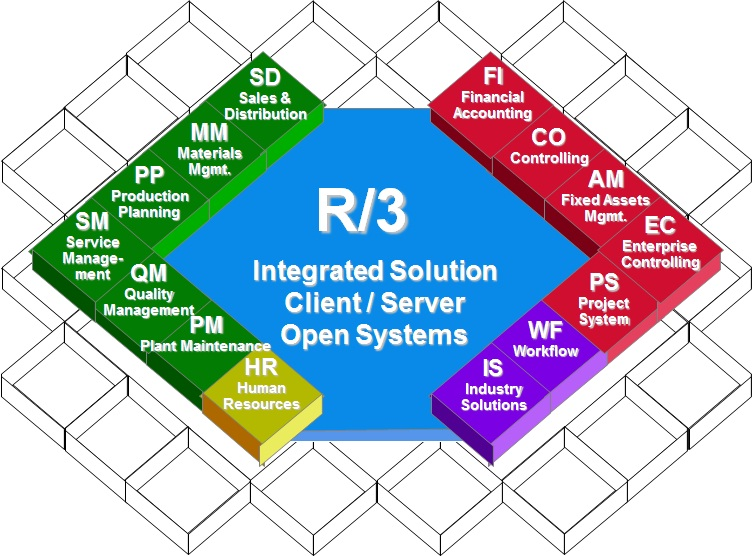
\includegraphics[width=1\textwidth]{images/sap_r3.jpg}
	\caption{Moduly SAP R3}
	\label{img:sapr3}
	\small
	fghfghgddh
\end{figure}

\begin{itemize}
	\item
	\textbf{Financial Accounting (FI)} označuje finanční účetnictví a je jedním z nejdůležitějších modulů SAP ERP. Používá se k uložení finančních dat organizace a pomáhá analyzovat finanční podmínky společnosti na trhu.
	\item
	\textbf{Controlling (CO)} podporuje koordinaci, monitorování a optimalizaci všech procesů v organizaci. Zahrnuje správu a konfiguraci základních dat, které pokrývají náklady a výnosy, interní objednávky a další nákladové prvky a funkční oblasti. Jeho hlavním účelem je plánování. Umožňuje určit odchylky srovnáním skutečných dat s údaji plánu a tím umožňuje řídit obchodní toky v organizaci.
	\item
	\textbf{Asset Management (AM)} slouží k optimální správě fyzického majetku organizace. Zahrnuje takové funkcionality jako jsou návrh, konstrukce, provoz, údržba a výměna zařízení. Spravuje majetek v jednotlivých odděleních (obchodních jednotkách).
	\item
	\textbf{Project system (PS)} - je nástroj pro správu dlouhodobých projektů. Umožňuje uživatelům plánovat finanční prostředky i zdroje a kontrolovat jednotlivé části projektu tak, aby bylo zaručeno včasné dodání pokud možno v rámci rozpočtu.
	\item
	\textbf{Workflow (WF)} - umožňuje navrhovat a realizovat obchodní procesy v rámci aplikačních systémů SAP. Zajišťuje aby se práce dostala v požadovaný čas do rukou správným lidem. Jeho cílem je usnadnění automatizace podnikových procesů.
	\item
	\textbf{Industry Solutions (IS)} - poskytuje specifická řešení pro desítky industriálních odvětví jako například pro automobilový, chemický či energetický průmysl.
	\item
	\textbf{Human Resources (HR)} - umožňuje organizaci strukturálně a efektivně zpracovávat informace údaje týkající se zaměstnanců k potřebám obchodním požadavkům.
	\item
	\textbf{Plant Maintenance (PM)} - poskytuje nástroj pro provádění veškerých potřebných činností týkajících se údržby organizace a jejích součástí. Umožňuje plánovat údržbu i s ohledem na materiálovou potřebu, zaznamenávat a vyrovnávat náklady spojené s činností.
	\item
	\textbf{Materials Management (MM)} - se zabývá řízením materiálů a skladových zásob. Kontroluje, aby nedocházelo k nedostatkům zboží a nevznikaly tak mezery v řetězci dodavatelského procesu.
	\item
	\textbf{Production Planning (PP)} - sleduje a zaznamenává toky ve výrobním procesu. Má za úkol sladění poptávky s výrovním kapacitou spolu s vytvořením plánů k dokončení komponentů a produktů.
	\item
	\textbf{Quality Management (QM)} - je modul úzce provázaný s moduly MM, PP či PM a nedílnou součástí logistického řízení. Používá se k prováděnější kvalitativních funkcí jako je plánovaní jakosti, zajištění a kontroly kvality ve výrobním a spotřebním procesu.
	\item
	\textbf{Sales and Distribution (SD)} - se používá pro ukládání údajů o zákaznících a produktech organizace. Pomáhá řídit fakturaci, prodej a přepravu produktů či služeb organizace. Řídí vztah se zákazníky od počáteční nabídky až po prodejní zakázku a fakturaci produktu.   
\end{itemize} 	

\section{SAP Plant Maintenance (PM)}
Modul SAP Plant Maintenance je komplexní řešení, které poskytuje nástroje pro kompletní údržbu v rámci firmy. Objekt údržby se skládá z technických objektů představujících strojní zařízení a skutečného modelu závodu.

Modul se skládá z činností jako je například správa technických objektů, zpracování údržby nebo preventivní údržba. Používá se k komplexnímu plánování, provádění denních činností údržby s integrací do ostatních SAP modulů.

\subsection{Technické objekty}
Pakliže je ve firmě zapotřebí správně nastavit DP (data processing) podporující údržbu, je nutné stávající technické systémy strukturovat na základě technických objektů. Vytvoření hierarchické podoby s sebou přináší následující výhody.
\begin{itemize}
	\item
	Doba potřebná pro správu technických objektů je snížena.
	\item
	Zpracování údržby je zjednodušeno.
	\item
	Doba strávená při zadávání dat během zpracování údržby je značně snížena.
	\item
	Konkrétnější, důkladnější a rychlejší vyhodnocení údajů o údržbě.
\end{itemize}

Technická správa objektů se skládá z následujících činností:
\begin{itemize}
	\item
	\textbf{Inspekce} - měřit a sledovat aktuální stav technického objektu
	\item
	\textbf{Preventivní údržba} - předvídat potřebu oprav a udržovat optimální stav technického objektu
	\item
	\textbf{Oprava} - měření a obnovení technického objektu
	\item
	\textbf{Další činnosti související s údržbou}
\end{itemize}
\vspace*{0.5cm}
Zpracování údržby pomáhá řídit skutečné údržbářské práce prováděné v údržbě. Proces se skládá ze tří oblastí:
\begin{itemize}
	\item
	\textbf{Upozornění na údržbu} -  oznamte poruchu nebo popište technickou podmínku objektu
	\item
	\textbf{Objednávka údržby} - provést podrobný plán údržby a sledovat průběh práce a uhradit náklady na údržbu
	\item
	\textbf{Historie údržby} - uložení důležitých údajů údržby pro vykazování a vyhodnocení
\end{itemize} 	

\subsection{Preventivní údržba}
Preventivní údržba je dlouhodobý proces, jehož cílem je zajistit vysokou použitelnost zařízení a funkčních míst a minimalizovat prostoje způsobené opravami. Tato funkce podporuje údržbu založenou na výkonu, pokud jsou měřicí body nebo čítače používány pro řízení technických podmínek objektu.
Součást preventivní údržby lze použít k:
\begin{itemize}
	\item
	Uložit seznam úkolů, které mají být provedeny
	\item
	Upřesněte rozsah inspekčních prací, preventivní údržbu a plánování činností
	\item
	Zadejte opakovanou frekvenci údržby
	\item
	Upřesněte přiřazení kontrolních činností a preventivní údržbu na základě nákladů
	\item
	Vyhodnotit náklady na budoucí preventivní údržbu a inspekční práci
\end{itemize} 	

Preventivní údržba v organizaci se používá k zabránění selhání systému a rozpadu výroby. Pomocí preventivní údržby můžete ve vaší organizaci dosáhnout různých výhod. Preventivní údržba se používá k provádění inspekcí, preventivní údržby a oprav. Plány údržby slouží k definování dat a rozsahu úkolů preventivní a inspekční údržby, které lze naplánovat pro technické objekty.

Seznam úkolů v Preventivní údržbě je definován jako sled činností, které jsou prováděny v rámci preventivní údržby v organizaci. Jsou používány k provádění opakovaných úkolů v rámci preventivní údržby a k jejich efektivnímu provedení.

Pomocí seznamů úkolů můžete snížit úsilí standardizací pracovní postup. Všechny aktualizace se provádějí na jednom konkrétním místě v seznamu úkolů údržby a všechny položky údržby a údržby v systému obdrží aktualizovaný stav pracovních postupů. Pomocí seznamů úkolů pomáhá při snižování úsilí potřebného pro vytvoření objednávek údržby a položek údržby, jak můžete vrátit do seznamu úkolů, abyste viděli pracovní postup.
Klíčové funkce seznamů úkolů v SAP Plant Maintenance jsou následující plánovaná a probíhající údržba podrobněji popsány v následujících odstavcích.

\paragraph{Plánovaná údržba}
Všechny plánované činnosti, jako je kontrola, údržba a opravy, jsou součástí plánované údržby. V údržbě rostlin definujete časové intervaly, kdy je třeba pracovní kroky provést a pracovní sekvence, ve kterých musí být provedeny. Seznamy úkolů jsou při plánování plánování údržby přiřazeny plánu údržby.

\paragraph{Probíhající údržba}
Seznam úkolů pro průběžnou údržbu obsahuje pracovní postupy založené na aktuální kontrole. Všechna kontrola, která se provádí bez pravidelného rozvrhu, je předmětem trvalé údržby.

\subsection{Zpracování údržby}
Zpracování údržby se skládá z několika úrovní, které nemusí být nutně plně realizovány.

Proto je možné zpracovat opravu v mnoha fázích plánování, jako je předběžná kalkulace, plánování práce, materiálové zabezpečení, plánování zdrojů a povolení. Je však také možné okamžitě reagovat na škody způsobené událostmi, které způsobí vypnutí výroby, a v co nejkratší možné době předložit požadované objednávky a prodejní doklady s minimálními údaji.

Zpracování údržby lze rozdělit na následující tři oblasti:
\begin{itemize}
	\item
	\textbf{Popis stavu objektu} - Nejdůležitějším prvkem v této oblasti je oznámení o údržbě. Používá se k popisu stavu technického objektu nebo hlášení poruchy na technickém objektu a požadavek na opravu poškození.
	\item
	\textbf{Provádění úkolů údržby} - Nejdůležitějším prvkem v této oblasti je objednávka údržby. Používá se k detailnímu plánování provádění údržbářských činností, sledování průběhu práce a vypořádání nákladů na údržbu.
	\item
	\textbf{Dokončení úkolů údržby} - Nejdůležitějším prvkem v této oblasti je historie údržby. Používá se k dlouhodobému uložení nejdůležitějších údajů o údržbě. Tyto údaje lze kdykoli vyžádat k vyhodnocení.
\end{itemize} 

Tyto prvky umožňují zpracovat všechny úkoly, které je třeba provést v údržbě zařízení, stejně jako operace, které nepatří přímo do údržby zařízení, jako jsou investice, restrukturalizace, úpravy a podobně.

\begin{figure}[H]
	\centering
	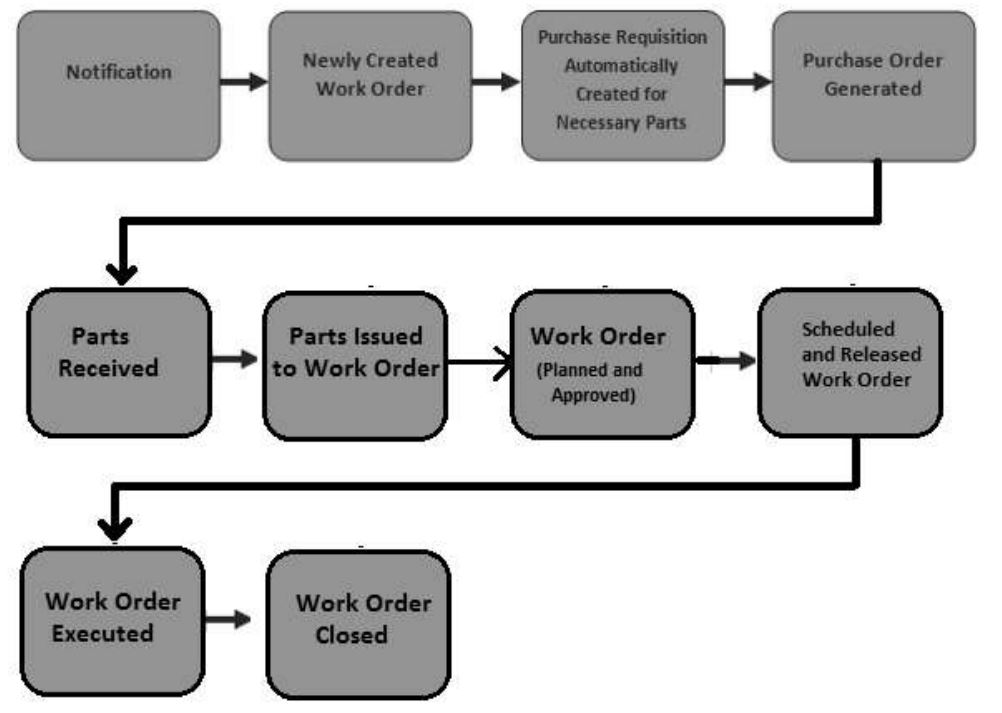
\includegraphics[width=1\textwidth]{images/pm_process.jpg}
	\caption{Proces diagram PM}
	\label{img:pm_process}
	\small
	Procesní diagram PM
\end{figure}

\section{SAP BSP}
Tato sekce se zaměřuje na front-endovou technologii SAP BSP. Jedná se o jednu z technologií použitých v cílové architektuře řešení mobilní aplikace a proto je zde stručně popsána její struktura.

\paragraph{SAP Web Application Server} SAP WAS je produktový produkt aplikačního serveru a nová generace produktu Basis. Poskytuje všechny funkce, které Basis udělal, a pak mnohem víc. Přemýšlejte o tom jako o nadpřirozené základně. Přemýšlejte o tom jako o obalení základny s obrovskými možnostmi webových aplikací, mezi které patří i schopnost spouštět aplikace Java / J2EE vedle aplikací ABAP. A chci říci, že přidání Java / J2EE k tomuto aplikačnímu serveru v žádném případě neohrožuje podporu pro ABAP. Všechny vaše investice do řešení ABAP jsou dobře chráněny. Rozdíl spočívá v tom, že oba vývojové a běhové prostředí ABAP a Java / J2EE se nacházejí na jedné platformě, na jedné společné infrastruktuře. Tato sjednocená oblast systému ABAP / Java minimalizuje úsilí učitele o výuku a náklady na správu.

\paragraph{BSP} Business Server Page (BSP) je kompletní funkční aplikace, stejně tak jako klasická transakce SAP. Rozhraním pro přístup však není software SAPGUI, spíše však libovolný webový prohlížeč. Díky využití protokolů HTTP nebo HTTPS je protokol používaný pro přístup k aplikaci po celé síti, což umožňuje používání standardních produktů, jako jsou firewally a proxy servery.

Programovací program Stránky Business Server je podobný technologii serverových stránek. Zaměřením programovacího modelu BSP jsou body, které zajišťují optimální strukturu v rozhraní a obchodní logiku.

\begin{figure}[H]
	\centering
	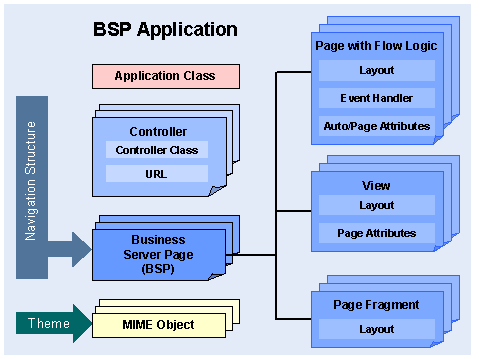
\includegraphics[width=1\textwidth]{images/bsp.png}
	\caption{Struktura BSP aplikace}
	\label{img:bsp}
	\small
	Struktura BSP aplikace
\end{figure}

\section{SAP FIORI}

Stejně jako každý jiný tradiční počítačový software byly také přístupné ERP systémy prostřednictvím grafického uživatelského rozhraní na stacionárních místech PC nebo notebooků. Vzhledem k rychlému vývoji mobilních zařízení očekává velké množství uživatelů zlepšení a příležitosti pro mobilní použití.

V minulosti, mnoho zákazníků SAP vyjádřili svou nespokojenost ohledně staromódní vzhled a dojem z obrazovek SAP, stejně jako nedostatek exkluzivního přístupu přes desktop GUI pro většinu operací (jako schvalování objednávky, vytvoření prodejní objednávky, samostatně výdělečně servisní úkoly, vyhledávání informací.) Zpětná vazba byla oceněna a SAP podnikla kroky ke zlepšení použitelnosti a dostupnosti. (Bince 2015, 365)
Dne 15. května 2013 představila společnost SAP platformu SAP Mobile Platform 3.0, otevřenou platformu, která byla k dispozici vývojářům softwaru. Společně se zavedením platformy zahájila společnost SAP svůj nový mobilní produkt s názvem Fiori. (SAP Fiori 2013, citováno 9. listopadu 2016.) Tento nový produkt je založen na pěti zásadách návrhu (obrázek 4).
Prostřednictvím tohoto nového mobilního řešení uživatelsky orientované klienti nyní měl přístup k novým řešením, kde sbírka aplikací bylo možné použít na různých zařízení, jako jsou stolní počítače, chytré telefony a tablety. V prvním vydání Flowers bylo zařazeno 25 aplikací, které slouží klientům v jejich nejčastějších obchodních funkcích. (SAP Fiori 2013, citováno 9. listopadu 2016.)


\begin{figure}[H]
	\centering
	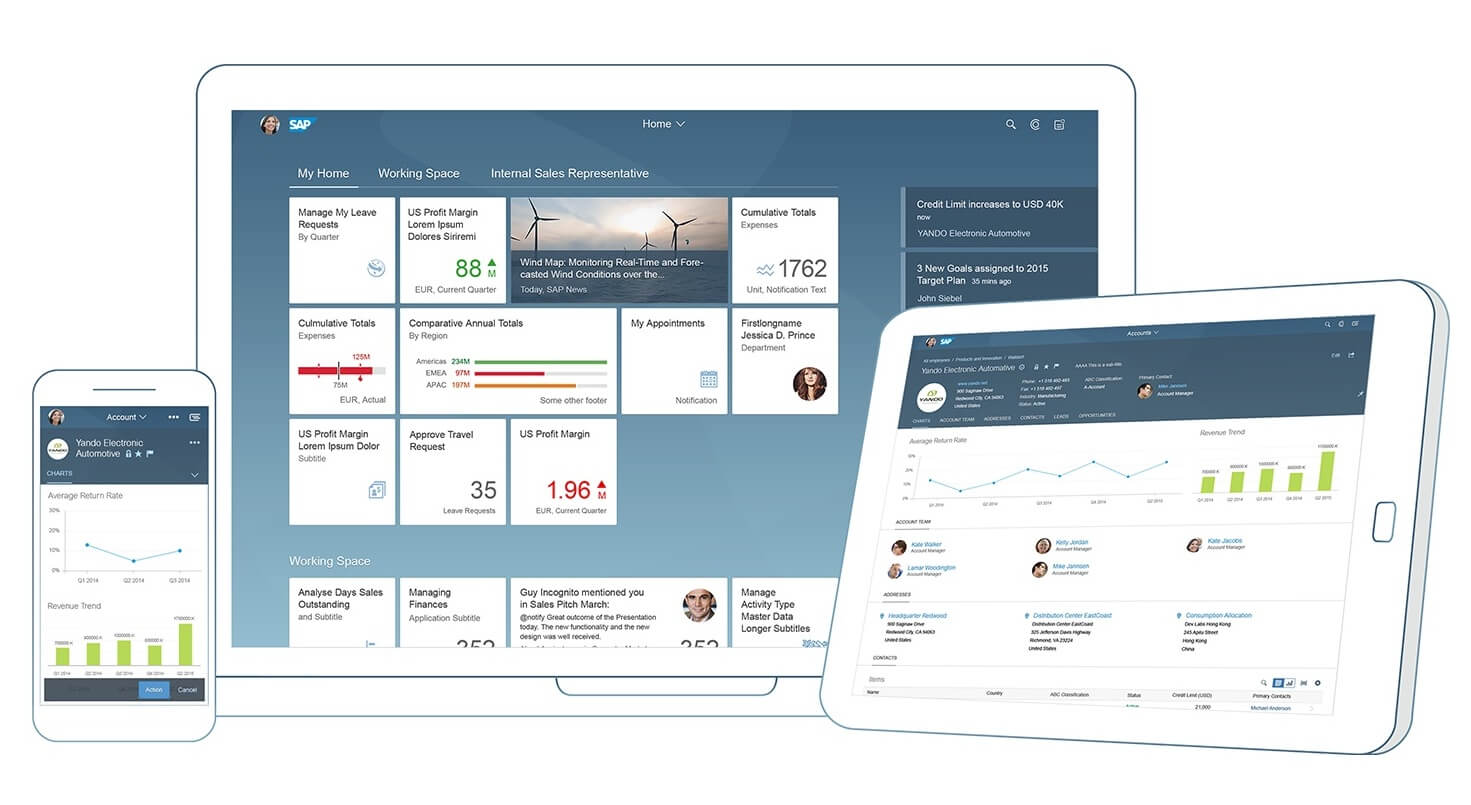
\includegraphics[width=1\textwidth]{images/fiori.jpg}
	\caption{Struktura BSP aplikace}
	\label{img:fiori}
	\small
	Struktura BSP aplikace
\end{figure}


\begin{itemize}
	\item
	Založené na rolích:
	- Uživatelsky orientované aplikace závislé na odpovědnosti uživatele
	- uživatel může mít více rolí a spouštět různé úkoly v několika doménách
	\item
	citlivý:
	- založené na formátu HTML5; pracuje bez problémů na různých zařízeních a velikostech obrazovky
	- automaticky upravuje rozložení aplikací na dostupné obrazovce
	- podporuje různé režimy interakce, jako klávesnice, myši a dotykové vstupy
	\item
	Jednoduché:
	- Jednoduché uživatelské rozhraní podporuje rychlé a snadné dokončení úkolů
	- má přístup 1: 1: 3: jeden uživatel, jeden případ, tři obrazovky (stolní, tabletové, mobilní)
	\item
	koherentní:
	- uživatel může mít mnoho aplikací, které mají stejný design a použitelnost
	- Snadno se naučíte nové aplikace poté, co se učíte používat jednu aplikaci Fiori
	\item
	Okamžitá hodnota:
	- stejný návrhový vzorec v aplikacích snižuje čas a náklady na školení nových uživatelů
\end{itemize} 	

\begin{figure}[H]
	\centering
	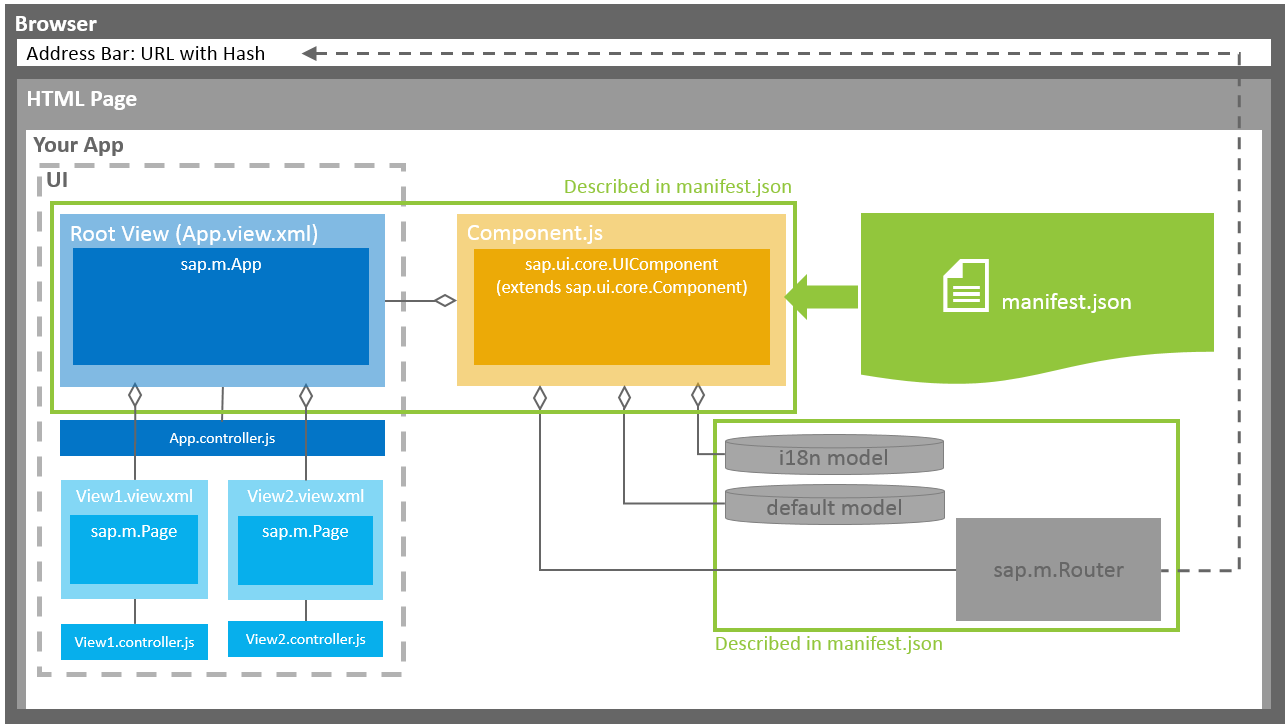
\includegraphics[width=1\textwidth]{images/fiori_arch.png}
	\caption{Struktura BSP aplikace}
	\label{img:fiori_arch}
	\small{ https://sapui5.hana.ondemand.com/\#/topic/28b59ca857044a7890a22aec8cf1fee9.html }
\end{figure}

\subsection{MVC}

\begin{figure}[H]
	\centering
	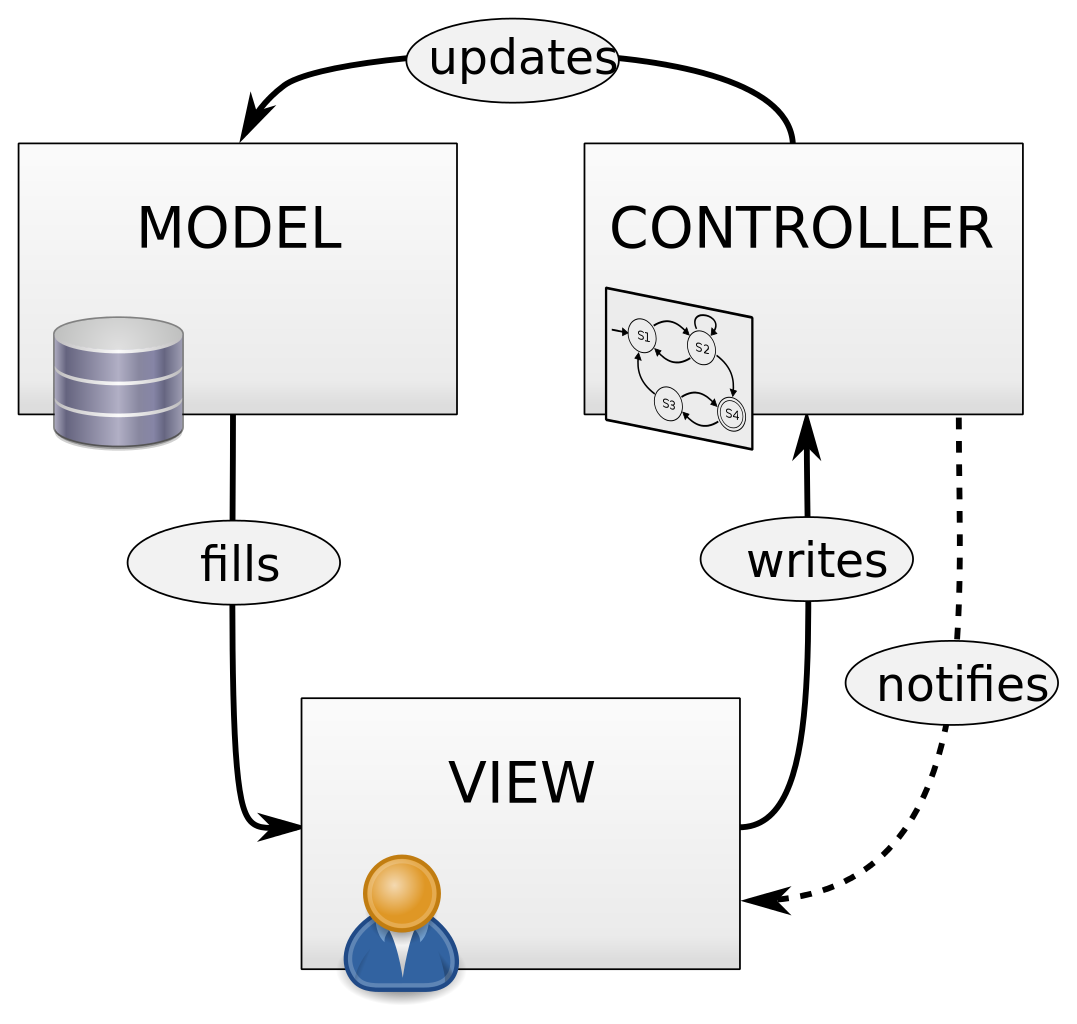
\includegraphics[width=0.6\textwidth]{images/mvc.png}
	\caption{Struktura BSP aplikace}
	\label{img:bsp}
	\small
	Struktura BSP aplikace
\end{figure}

\paragraph{Model} reprezentuje správu vlastních dat, nad nimiž aplikace pracuje: to mů-že být třeba obrázek, textový dokument, databáze uložená na serveru SQL, … Je dobré si uvědomit rozdíl mezi daty samotnými a jejich správcem (tedy prá-vě tím modelem, o němž zde hovoříme). Třeba takový konkrétní obrázek jsou data; skupina tříd, umožňující obrázky načítat ze souborů a opět do nich uklá-dat, zjišťovat a měnit jejich atributy, převádět jejich formáty a pracovat s jejich obsahem – to je správce. V běžící aplikaci pak samozřejmě bude základním ob-jektem vrstvy modelu nějaká vhodná instance, jež bude reprezentovat vlastní obrázek a nabízet všechny odpovídající služby.

\paragraph{View} zahrnuje všechny objekty (grafického) uživatelského rozhraní a jejich služby. Uživatel aplikace s ní komunikuje výhradně prostřednictvím těchto ob-jektů; právě ony mu prezentují data z modelu ve vhodné formě, a naopak pou-ze jejich prostřednictvím uživatel dává aplikaci příkazy, jež určují její další činnost.
View má s modelem společnou tu nejdůležitější věc: jeho objekty nejsou závislé na konkrétní aplikační logice. Grafické uživatelské rozhraní aplikace tak mů-žeme podle potřeby (a podle požadavků zákazníků) snadno kdykoliv měnit, aniž by bylo zapotřebí přitom nějak zasahovat do aplikační logiky (nebo do-konce do modelu).

\paragraph{Controller} mezi datovým modelem a objekty grafického uživatelského roz-hraní, jež tvoří vzhled, stojí vrstva controller; právě na její úrovni je imple-mentována funkční logika aplikace, takové věci jako „stiskne-li uživatel tohle tlačítko, provede se támhleta akce, a v tomto textovém poli se zobrazí výsle-dek“. (Čada, 2009)

\begin{figure}[H]
	\centering
	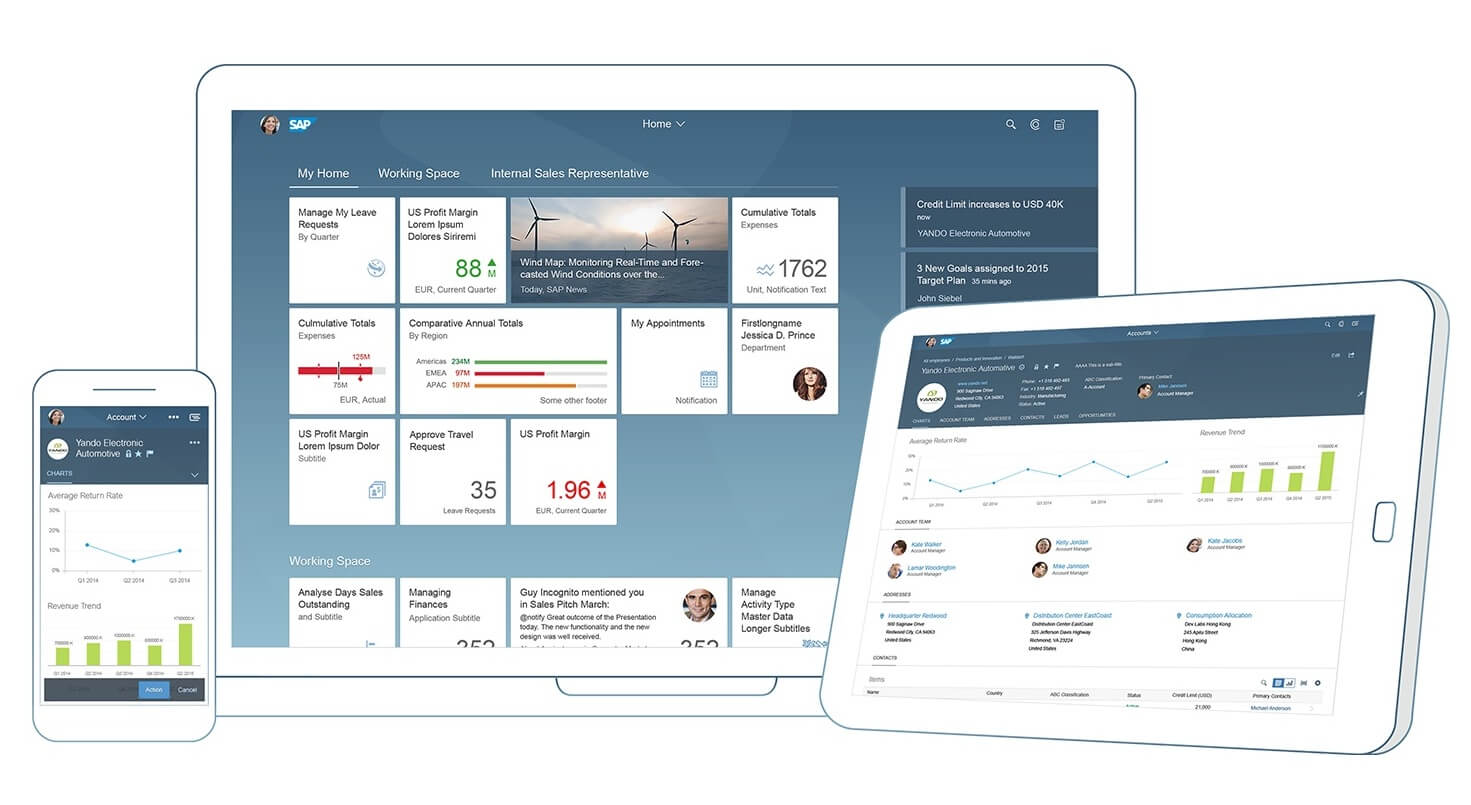
\includegraphics[width=1\textwidth]{images/fiori.jpg}
	\caption{Struktura BSP aplikace}
	\label{img:fiori}
	\small
	Struktura BSP aplikace
\end{figure}

\subsection{SAP ODATA}

\paragraph{Protokol OData} umožňuje vytváření datových služeb založených na webovém protokolu REST (representational state transfer), který umožňuje uživatelům provádět CRUDQ operace nad zdroji identifikovanými pomocí Uniform Resource Identifier (URI) a definovanými v datovém modelu použitím jednoduchých HTTP zpráv.

Protokol původně vyvinul Microsoft, verze 1.0, 2.0 a 3.0 jsou uvolněny pod Microsoft Open Specification Promise. Aktuálně nejnovější verze 4.0 byla schválena jako standard prostřednictvím OASIS OData Technical Committee, jejímiž členy jsou BlackBerry, IBM, Microsoft, SAP a další. Následující informace ohledně OData protokolu se budou vztahovat k verzi 2.0, která je momentálně v SAPu navzdory zavádění verze 4.0, používána nejčastěji. 

Data přenášená prostřednictvím OData protokolu mohou využívat různé datové formáty běžně používané ve webových technologiích, například Extensible Markup Language (XML), JavaScript Object Notation (JSON) nebo Atom Publishing Pro-tocol (AtomPub) a další. Data jsou při přenosu zabalena do protokolu HTTP, případně do jeho zabezpečené verze HTTPS.

Jádrem OData jsou feeds, které jsou kolekcemi Collections složené ze záznamů Entries. Každý Entry je identifikovaný klíčem a reprezentuje strukturovaný záznam, který má seznam vlastností Properties, ty mohou být komplexního, nebo primitivního typu. Entries mohou být součástí hierarchie typů a mohou mít související entries a feeds odkazované prostřednictvím Links.

\paragraph{Metadata} OData služba poskytuje metadata dokumenty. Aby mohli uživatelé oData služby prozkoumat, co všechno služba nabízí, aniž by museli zkoumat implementaci služ-by na backendu.
Jednodušší Service Document se nachází v root URI služby, obsahuje seznam všech feedů, takže je uživatelé mohou prozkoumat a zjistit jejich adresy.
Přidáním segmentu \$metadata do root URI služby získáme Service Metadata Document, který popisuje celý datový model, jinými slovy strukturu a propojení všech zdrojů. Jak uvádí (Odata, 2013), Service Metadata Document popisuje svá data pomocí termínů EDM použitím XML jazyka pro popis modelů nazvaných Con-ceptual Schema Definition Language (CSDL). Tento CSDL dokument je pak zabalen použitím formátu EDMX. (Odata, 2015)

\paragraph{Entity Data Model (EDM)} Hlavním konceptem v EDM jsou entity a asociace. Entity jsou instance Entity Type (například Inventura, Závod, Budova a tak dále), které jsou strukturovanými zá-znamy s klíčem Entity Key a složenými z pojmenovaných a typovaných vlastností. Entity Key je složen z podmnožiny vlastností v Entity Type. Entity Key (například InventuraID, nebo BudovaID) je zásadní koncept pro unikátní identifikaci instancí Entity Type a umožnění Enity Type instancím fungovat ve vztazích. Entity jsou se-skupovány v Entity Sets (například Budovy je množina instancí Entity Type Budo-va).
Asociace definují vztah mezi dvěma nebo více Enity Type (například Budova patří Závodu). Instance asociací jsou seskupovány v Association Sets. Navigation Properties jsou speciální vlastnosti v Entity Type, které jsou vázány na konkrétní asociaci a mohou být použity k odkazování na asociaci entity.
Položením předchozích definic do OData termínů, feedy vystavované OData službou jsou reprezentovány pomocí Entity Set, nebo Navigation Property na Entity Type, které identifikuje kolekci entit. Například Entity Set identifikovaný pomocí URI http://services.odata.org/OData/OData.svc/Products, nebo kolekce entit identifikovaná pomocí Products Navigation Property v http://services.odata.org/OData/OData.svc/Categories(1)/Products identifikují feed složený z Entry vystavovaný OData službou. (Odata, 2015)

\begin{figure}[H]
	\centering
	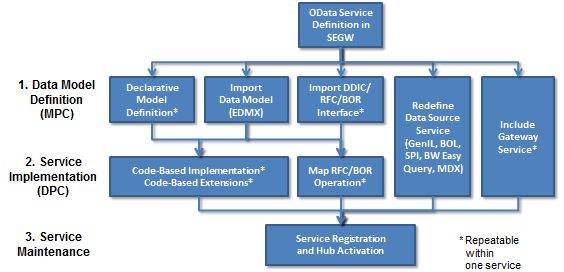
\includegraphics[width=1\textwidth]{images/odata.png}
	\caption{Struktura BSP aplikace}
	\label{img:bsp}
	\small
	Struktura BSP aplikace
\end{figure}

\chapter{Analýza a návrh aplikace}
Tato kapitola se věnuje analýze mnou navrženého řešení. Obsahuje jednotlivé podkapitoly zaměřující se na zpracování požadavků kladených na výslednou aplikaci, funkčnost RFID čtečky i návrh kompletního třídního modelu.	

\section{Model požadavků}
V této kapitole jsou uvedeny veškeré požadavky kladené na  výslednou aplikaci, které byly probírány se zadavatelem. Většina z nich byla stanovena ihned po určení rámcového zadání, některé však byly přidány nebo lehce upraveny v rámci konzultací , jak se upravovalo zadání práce. Následující výčet požadavků je rozdělen do dvou kategorií a to do funkčních a nefunkčních požadavků.  

\subsection{Funkční požadavky}
Funkční požadavky jsou rozděleny do 8 sekcí označených jako F1 až F8. 

\subsubsection{F1: Založení poruchy}
\subsubsection{F2: Založení požadavku na údržbu}
\subsubsection{F3: Zobrazení seznamu aktivních poruch}
\subsubsection{F4: Zobrazení seznamu historie poruch}
\subsubsection{F5: Zobrazení seznamu požadavků na údržbu}
\subsubsection{F6: Zobrazení seznamu prevencí}
\subsubsection{F7: Zobrazení dokumentace ke stroji (vybavení)}
\subsubsection{F8: Administrace uživatele}


\subsection{Nefunkční požadavky}

\subsubsection{N1: Grafické uživatelské rozhraní}
\subsubsection{N2: Provoz na provozních počítačích}
\subsubsection{N3: Provoz na mobilních zařízeních}
\subsubsection{N4: Dostupnost přes web}

\section{Model případů užití (Use Case model)}
Detailní specifikace funkčních požadavků, Typicky se jednotlivé požadavky rozpadají na několik případů užití. Základ pro tvorbu uživatelské příručky
– Podklady k tvorbě akceptačních testů
– Zpřesnění odhadů pracnosti
– Zadání pro programátora


\subsection{Seznam účastníků}

\begin{itemize}
	\item
	\textbf{Operátor výroby} - 
	\item
	\textbf{Údržbář} - 
	\item
	\textbf{Správce / Administrátor} - 
\end{itemize} 	

\subsection{Diagram případů užití}

\subsubsection{UC1: Vložit novou knihu}

\section{Návrh uživatelského rozhraní}

\subsection{Heuristická analýza}
Při návrhu uživatelského rozhraní je dobré držet se deseti následujících pravidel z Nielsenovi heuristické analýzy. V této kapitole je čerpáno ze zdrojů [8] a [9]. Nielsenova heuristická analýza je jednou ze základních metod pro testování uživatelského rozhraní. Jedná se o seznam pravidel, které by mělo uživatelské rozhraní splňovat. Jakob Nielsen a Rolf Molich v roce 1990 vytvořili heuristiku
pro heuristické vyhodnocení a poté v roce 1994 Jakob Nielsen revidoval tuto heristiku na množinu pravidel.

\begin{enumerate}
	\item
	\textbf{Viditelnost stavu systému} - Uživatel by měl být vždy systémem vhodně informován (v rozumném čase)
	o tom co se zrovna děje. Systém by tak měl reagovat na uživatelský vstup, nebo v případě, že se například provádí nějaký časově náročnější výpočet nebo
	stahování dat, tak zobrazit progress bar.
	\item
	\textbf{Propojení systému a reálného světa} - Systém by měl na uživatele mluvit jazykem uživatele se slovy, frázemi a koncepty, které jsou uživateli známé, zná je z reálného světa. Neměly by se využívat
	pojmy, které jsou například specifické pouze pro daný systém.
	\item
	\textbf{Uživatelská kontrola a svoboda} - Uživatelé se často učí nové funkce systému pomocí chyb, které provedou. Když uživatelé udělají chybu, musí mít možnost provedenou akci vrátit zpět a vrátit
	tak systém do předchozího stavu. V případě, že se provádí nenávratná akce,
	je třeba na to uživatele řádně upozornit.
	\item
	\textbf{Standardizace a konzistence} - Uživatel nesmí být zmaten různými termíny v různých situacích, přestože mají dané termíny stejný význam. Systém by měl vždy dodržovat standardy, které
	jsou na dané platformě. Proto je například potřeba dodržovat standardní chybové
	hlášky, správné umístění komponent apod. Ideální je používat standardní
	platformové komponenty.
	\item
	\textbf{Prevence chyb} - Lepší než dobré chybové hlášky je návrh, který zabraňuje samotnému výskytu
	chyb. Buď je možné podmínky náchylné k chybám co nejvíce eliminovat, nebo
	na chyby uživatele upozornit ještě dříve než například potvrdí formulář.
	\item
	\textbf{Rozpoznání namísto vzpomínání} - Je třeba minimalizovat zatěžování paměti uživatele tím, že uživatel vždy vidí potřebné informace a akce, které může provést. Uživatel si tak například nemusí
	pamatovat informace z jedné části formuláře na další.
	\item
	\textbf{Flexibilní a efektivní použití} - Systém by měl v závislosti na jeho možnostech a typu umožňovat dvě verze ovládání. Pro méně zkušené uživatele a pro zkušené uživatele. Verze pro méně zkušené uživatele by měla obsahovat pouze základní funkce a možnosti nastavení tak, aby „nezkušený“ uživatel nebyl zbytečně zatěžován funkcionalitami, které stejně nepotřebuje. Naopak pro zkušené uživatele by se	měli zobrazit všechny funkcionality, včetně těch složitějších. Zkušenější uživatel by měl mít také případně možnost si potřebné funkcionality přizpůsobit pomocí maker. Pro oba typy uživatelů je také dobré umožnit využívat klávesové zkratky
	\item
	\textbf{Estetický a minimalistický} - Uživatel by měl mít co nejméně možností kam může kliknout, protože každá
	další možnost soutěží o pozornost uživatele. Čím méně možností uživatel má,
	tím rychleji je schopen pokračovat. Na obrazovce by také měly být zobrazeny
	pouze informace, které uživatel v dané situaci opravdu potřebuje.
	\item
	\textbf{Pomoc uživatelů pochopit, poznat a vzpamatovat se z chyb} - Chybové hlášky by měly být v přirozeném jazyce a neměly by například obsahovat
	žádné chybové kódy apod. Hlášky by měly přesně popisovat co je za
	problém a doporučit uživateli jak pokračovat dál. Ideální je, když uživatel
	nemá možnost dojít do stavu, kdy je potřeba chybové hlášení.
	\item
	\textbf{Nápověda a návody} - Přestože je lepší, když je systém použitelný bez jakékoliv nápovědy, nápovědu
	by měl systém obsahovat. Veškeré informace by v systému měly být snadno
	vyhledatelné a obsahem nápovědy by měly být názorné příklady.
\end{enumerate} 

\subsection{Lo-Fi prototyp}

\paragraph{Úvodní obrazovka}

\subsubsection{Balsamiq}

\subsubsection{Built}


\chapter{Návrh architektury}



\chapter{Implementace}

\section{Porovnání vývojových prostředí}

\section{Doporučení pro vývoj}

\begin{conclusion}
	%sem napište závěr Vaší práce
\end{conclusion}

\bibliographystyle{csn690}
\bibliography{mybibliographyfile}

\appendix

\chapter{Seznam použitých zkratek}
% \printglossaries
\begin{description}
	\item[GUI] Graphical user interface
	\item[XML] Extensible markup language
\end{description}


% % % % % % % % % % % % % % % % % % % % % % % % % % % % 
% % Tuto kapitolu z výsledné práce ODSTRAŇTE.
% % % % % % % % % % % % % % % % % % % % % % % % % % % % 
% 
% \chapter{Návod k~použití této šablony}
% 
% Tento dokument slouží jako základ pro napsání závěrečné práce na Fakultě informačních technologií ČVUT v~Praze.
% 
% \section{Výběr základu}
% 
% Vyberte si šablonu podle druhu práce (bakalářská, diplomová), jazyka (čeština, angličtina) a kódování (ASCII, \mbox{UTF-8}, \mbox{ISO-8859-2} neboli latin2 a nebo \mbox{Windows-1250}). 
% 
% V~české variantě naleznete šablony v~souborech pojmenovaných ve formátu práce\_kódování.tex. Typ může být:
% \begin{description}
% 	\item[BP] bakalářská práce,
% 	\item[DP] diplomová (magisterská) práce.
% \end{description}
% Kódování, ve kterém chcete psát, může být:
% \begin{description}
% 	\item[UTF-8] kódování Unicode,
% 	\item[ISO-8859-2] latin2,
% 	\item[Windows-1250] znaková sada 1250 Windows.
% \end{description}
% V~případě nejistoty ohledně kódování doporučujeme následující postup:
% \begin{enumerate}
% 	\item Otevřete šablony pro kódování UTF-8 v~editoru prostého textu, který chcete pro psaní práce použít -- pokud můžete texty s~diakritikou normálně přečíst, použijte tuto šablonu.
% 	\item V~opačném případě postupujte dále podle toho, jaký operační systém používáte:
% 	\begin{itemize}
% 		\item v~případě Windows použijte šablonu pro kódování \mbox{Windows-1250},
% 		\item jinak zkuste použít šablonu pro kódování \mbox{ISO-8859-2}.
% 	\end{itemize}
% \end{enumerate}
% 
% 
% V~anglické variantě jsou šablony pojmenované podle typu práce, možnosti jsou:
% \begin{description}
% 	\item[bachelors] bakalářská práce,
% 	\item[masters] diplomová (magisterská) práce.
% \end{description}
% 
% \section{Použití šablony}
% 
% Šablona je určena pro zpracování systémem \LaTeXe{}. Text je možné psát v~textovém editoru jako prostý text, lze však také využít specializovaný editor pro \LaTeX{}, např. Kile.
% 
% Pro získání tisknutelného výstupu z~takto vytvořeného souboru použijte příkaz \verb|pdflatex|, kterému předáte cestu k~souboru jako parametr. Vhodný editor pro \LaTeX{} toto udělá za Vás. \verb|pdfcslatex| ani \verb|cslatex| \emph{nebudou} s~těmito šablonami fungovat.
% 
% Více informací o~použití systému \LaTeX{} najdete např. v~\cite{wikilatex}.
% 
% \subsection{Typografie}
% 
% Při psaní dodržujte typografické konvence zvoleného jazyka. České \uv{uvozovky} zapisujte použitím příkazu \verb|\uv|, kterému v~parametru předáte text, jenž má být v~uvozovkách. Anglické otevírací uvozovky se v~\LaTeX{}u zadávají jako dva zpětné apostrofy, uzavírací uvozovky jako dva apostrofy. Často chybně uváděný symbol "{} (palce) nemá s~uvozovkami nic společného.
% 
% Dále je třeba zabránit zalomení řádky mezi některými slovy, v~češtině např. za jednopísmennými předložkami a spojkami (vyjma \uv{a}). To docílíte vložením pružné nezalomitelné mezery -- znakem \texttt{\textasciitilde}. V~tomto případě to není třeba dělat ručně, lze použít program \verb|vlna|.
% 
% Více o~typografii viz \cite{kobltypo}.
% 
% \subsection{Obrázky}
% 
% Pro umožnění vkládání obrázků je vhodné použít balíček \verb|graphicx|, samotné vložení se provede příkazem \verb|\includegraphics|. Takto je možné vkládat obrázky ve formátu PDF, PNG a JPEG jestliže používáte pdf\LaTeX{} nebo ve formátu EPS jestliže používáte \LaTeX{}. Doporučujeme preferovat vektorové obrázky před rastrovými (vyjma fotografií).
% 
% \subsubsection{Získání vhodného formátu}
% 
% Pro získání vektorových formátů PDF nebo EPS z~jiných lze použít některý z~vektorových grafických editorů. Pro převod rastrového obrázku na vektorový lze použít rasterizaci, kterou mnohé editory zvládají (např. Inkscape). Pro konverze lze použít též nástroje pro dávkové zpracování běžně dodávané s~\LaTeX{}em, např. \verb|epstopdf|.
% 
% \subsubsection{Plovoucí prostředí}
% 
% Příkazem \verb|\includegraphics| lze obrázky vkládat přímo, doporučujeme však použít plovoucí prostředí, konkrétně \verb|figure|. Například obrázek \ref{fig:float} byl vložen tímto způsobem. Vůbec přitom nevadí, když je obrázek umístěn jinde, než bylo původně zamýšleno -- je tomu tak hlavně kvůli dodržení typografických konvencí. Namísto vynucování konkrétní pozice obrázku doporučujeme používat odkazování z~textu (dvojice příkazů \verb|\label| a \verb|\ref|).
% 
% \begin{figure}\centering
% 	
\includegraphics[width=0.5\textwidth, angle=30]{cvut-logo-bw}
% 	\caption[Příklad obrázku]{Ukázkový obrázek v~plovoucím prostředí}\label{fig:float}
% \end{figure}
% 
% \subsubsection{Verze obrázků}
% 
% % Gnuplot BW i barevně
% Může se hodit mít více verzí stejného obrázku, např. pro barevný či černobílý tisk a nebo pro prezentaci. S~pomocí některých nástrojů na generování grafiky je to snadné.
% 
% Máte-li například graf vytvořený v programu Gnuplot, můžete jeho černobílou variantu (viz obr. \ref{fig:gnuplot-bw}) vytvořit parametrem \verb|monochrome dashed| příkazu \verb|set term|. Barevnou variantu (viz obr. \ref{fig:gnuplot-col}) vhodnou na prezentace lze vytvořit parametrem \verb|colour solid|.
% 
% \begin{figure}\centering
% 	\includegraphics{gnuplot-bw}
% 	\caption{Černobílá varianta obrázku generovaného programem Gnuplot}\label{fig:gnuplot-bw}
% \end{figure}
% 
% \begin{figure}\centering
% 	\includegraphics{gnuplot-col}
% 	\caption{Barevná varianta obrázku generovaného programem Gnuplot}\label{fig:gnuplot-col}
% \end{figure}
% 
% 
% \subsection{Tabulky}
% 
% Tabulky lze zadávat různě, např. v~prostředí \verb|tabular|, avšak pro jejich vkládání platí to samé, co pro obrázky -- použijte plovoucí prostředí, v~tomto případě \verb|table|. Například tabulka \ref{tab:matematika} byla vložena tímto způsobem.
% 
% \begin{table}\centering
% 	\caption[Příklad tabulky]{Zadávání matematiky}\label{tab:matematika}
% 	\begin{tabular}{|l|l|c|c|}\hline
% 		Typ		& Prostředí		& \LaTeX{}ovská zkratka	& \TeX{}ovská zkratka	\tabularnewline \hline \hline
% 		Text		& \verb|math|		& \verb|\(...\)|	& \verb|$...$|		\tabularnewline \hline
% 		Displayed	& \verb|displaymath|	& \verb|\[...\]|	& \verb|$$...$$|	\tabularnewline \hline
% 	\end{tabular}
% \end{table}
% 
% % % % % % % % % % % % % % % % % % % % % % % % % % % % 

\chapter{Obsah přiloženého CD}

%upravte podle skutecnosti

\begin{figure}
	\dirtree{%
		.1 readme.txt\DTcomment{stručný popis obsahu CD}.
		.1 exe\DTcomment{adresář se spustitelnou formou implementace}.
		.1 src.
		.2 impl\DTcomment{zdrojové kódy implementace}.
		.2 thesis\DTcomment{zdrojová forma práce ve formátu \LaTeX{}}.
		.1 text\DTcomment{text práce}.
		.2 thesis.pdf\DTcomment{text práce ve formátu PDF}.
		.2 thesis.ps\DTcomment{text práce ve formátu PS}.
	}
\end{figure}

\end{document}
